\documentclass[table]{magicstyle/magic}
\usepackage{amssymb}
\usepackage{multirow}
\usepackage{bigdelim}
\usepackage{todonotes}
\usepackage{longtable}
\usepackage{tabularray}
\usepackage{wrapfig}
\usepackage[most]{tcolorbox} 
\usepackage{url}
\usepackage{xspace}
\usepackage{svg}
\usepackage[absolute]{textpos} %
\usepackage{fdsymbol}   %
\usepackage{csvsimple}
\usepackage{nicematrix}
\newcolumntype{L}[1]{>{\raggedright\let\newline\\\arraybackslash\hspace{0pt}}m{#1}}
\newcolumntype{C}[1]{>{\centering\let\newline\\\arraybackslash\hspace{0pt}}m{#1}}
\newcolumntype{R}[1]{>{\raggedleft\let\newline\\\arraybackslash\hspace{0pt}}m{#1}}
% \newcolumntype{P}{>{\columncolor{ai2lightpink}}c}
\newcolumntype{P}[1]{>{\centering\let\newline\\\arraybackslash\columncolor{ai2lightpink}}m{#1}}
% \newcolumntype{W}[1]{>{\columncolor{white}}c}  % White column type for the first column
\addtolength{\extrarowheight}{\belowrulesep}
\aboverulesep=0pt
\belowrulesep=0pt


\newcommand{\taskitem}[4]{%
    \item \textbf{Task Name:} #1 \\
    \textbf{Task Description:} #2 \\
    \textbf{Language Description:} #3 \\
    \textbf{Task Progression Score Metrics:} #4
}
\usepackage{booktabs}              % \toprule, \midrule, \bottomrule
\usepackage{adjustbox}             % \begin{adjustbox}
\usepackage[dvipsnames,table]{xcolor}  % ForestGreen + \cellcolor
\usepackage[utf8]{inputenc} %
\usepackage[T1]{fontenc}    %
\usepackage{url}            %
\usepackage{booktabs}       %
\usepackage{amsfonts}       %
\usepackage{nicefrac}       %
\usepackage{microtype}      %
\usepackage[table]{xcolor}         %
\usepackage{amsmath}
\usepackage[most]{tcolorbox}
\usepackage{csquotes}

\usepackage{siunitx}
\usepackage{graphicx}
\usepackage{arydshln}
\usepackage{wrapfig}
\usepackage{enumitem}
\usepackage{soul} %

\usepackage{booktabs}
\usepackage{multirow}
\usepackage{threeparttable}
\usepackage{multirow}
\usepackage{xspace}
\usepackage{adjustbox}
\usepackage{pifont}
\usepackage{caption}
\usepackage{makecell}
\usepackage{subcaption}
\usepackage{bold-extra}
\usepackage{url}

\usepackage{booktabs,rotating,xcolor}


\usepackage{hyperref}
\definecolor{linkcolor}{HTML}{1F5A93}
\hypersetup{
     colorlinks   = true,
     citecolor    = linkcolor,
     linkcolor    = linkcolor,
     urlcolor     = linkcolor,
}
\usepackage{pifont}%
\newcommand{\cmark}{\ding{51}}%
\newcommand{\xmark}{\ding{55}}%
\usepackage{listings}
\usepackage{booktabs}
\usepackage{multirow}
\usepackage{rotating}
\usepackage{makecell}
\usepackage{array}
\setlist[itemize]{leftmargin=*,itemsep=0em,parsep=0.3em,topsep=0.3em}

\usepackage{array}  % in your preamble, if not already loaded\usepackage{array}  % in your preamble, if not already loaded

\addtolength{\extrarowheight}{\belowrulesep}
\aboverulesep=0pt
\belowrulesep=0pt

\usepackage{tikz}
\newcommand{\cblock}[3]{
  \hspace{-1.5mm}
  \begin{tikzpicture}
    [
    node/.style={square, minimum size=10mm, thick, line width=0pt},
    ]
    \node[fill={rgb,255:red,#1;green,#2;blue,#3}] () [] {};
  \end{tikzpicture}%
}

\newcommand{\norm}[1]{\left\lVert#1\right\rVert}

\definecolor{maroon}{HTML}{F26035}
\definecolor{yellow}{HTML}{FDBC42}
\definecolor{darkred}{RGB}{156, 39, 33}
\definecolor{darkblue}{RGB}{31, 90, 153}
\definecolor{forestgreen}{rgb}{0.13, 0.55, 0.13}


\newcommand{\missing}{\color{red}{xxx}\xspace}

% ---------------------------------------------------------------------------
% Project-specific macros. Rename these for your own paper.
% (The original MolmoAct2 paper macros are preserved in the git history.)
% ---------------------------------------------------------------------------
\newcommand{\methodname}{\textsc{MethodName}\xspace}
\newcommand{\datasetname}{\textsc{DatasetName}\xspace}

% Inline editing / review note, e.g. \todonote{double-check this number}
\newcommand{\todonote}[1]{{\color{orange} [note: #1]}}


\newcommand{\huggingface}{\raisebox{-1.5pt}{
\includegraphics[height=1.05em]{logos/hf.pdf}}\xspace}
\newcommand{\emailLogo}{\raisebox{-1.5pt}{
\includegraphics[height=1.05em]{logos/email.pdf}}\xspace}
\newcommand{\hfdataset}{\raisebox{-1.5pt}{
\includegraphics[height=1.05em]{logos/db.pdf}}\xspace}
\newcommand{\github}{\raisebox{-1.5pt}{
\includegraphics[height=1.05em]{logos/github.pdf}}\xspace}
\newcommand{\aitoo}{\raisebox{-1.5pt}{
\includegraphics[height=1.05em]{logos/magic-logo.png}}\xspace}
\newcommand{\wandb}{\raisebox{-1.5pt}{
\includegraphics[height=1.05em]{logos/wandb-logo.pdf}}\xspace}



  

\usepackage{setspace}
\usepackage{quoting}      % nice quote environment

\usepackage{nicematrix}
\newcolumntype{L}[1]{>{\raggedright\let\newline\\\arraybackslash\hspace{0pt}}m{#1}}
\newcolumntype{C}[1]{>{\centering\let\newline\\\arraybackslash\hspace{0pt}}m{#1}}
\newcolumntype{R}[1]{>{\raggedleft\let\newline\\\arraybackslash\hspace{0pt}}m{#1}}
\newcolumntype{P}[1]{>{\centering\let\newline\\\arraybackslash\columncolor{ai2lightpink}}m{#1}}
\newcolumntype{W}[1]{>{\columncolor{white}}c}  %
\addtolength{\extrarowheight}{\belowrulesep}
\aboverulesep=0pt
\belowrulesep=0pt

\newcommand{\aitwo}{\raisebox{-1.5pt}{
\includegraphics[height=1.05em]{logos/magic-logo.png}}\xspace}



\title{Paper Title\\{\fontsize{18pt}{12pt}\selectfont An Optional Descriptive Subtitle}}



\newcommand{\core}{\textsuperscript{\textcolor{ai2pink}{\ding{170}}}}
\authorOne[1*]{First Author\core}
\authorOne[1*]{Second Author\core}

\authorTwo[1]{Third Author}
\authorTwo[1]{Fourth Author}
\authorTwo[2]{External Collaborator}

\authorThree[1]{Jiafei Duan}

\affiliation[1]{MAGIC Lab, National University of Singapore}
\affiliation[2]{Collaborating Institution}

\contribution[]{
* denotes equal contribution. $\textcolor{ai2pink}{\varheartsuit}$ marks core contributors. Correspondence to \email{duanj1@nus.edu.sg}.
}

\abstract{

The abstract is a single paragraph of 4--6 sentences. State the problem and why it matters, what is missing in current approaches, what you propose (\method), and the main result with a concrete number (e.g., ``\method improves real-world success rate by 25\% over the strongest baseline''). End with what you release (code, models, data), if anything. Do not cite references or use undefined abbreviations in the abstract.

}


\metadata[\quad\github Code:]{
    \href{https://github.com/MAGICLAB-NUS}{\texttt{github.com/MAGICLAB-NUS}}
}

\metadata[\vspace{.5em}\quad\huggingface Models:]{
\href{https://huggingface.co/}{\texttt{your-org/your-model}}
}

\metadata[\vspace{.5em}\quad\hfdataset Data:]{
\href{https://huggingface.co/}{\texttt{your-org/your-dataset}}
}

\metadata[\vspace{.5em}\quad\aitoo Project page:]{\href{https://magiclab-nus.github.io/}{\texttt{magiclab-nus.github.io}}}

\correspondence{\email{duanj1@nus.edu.sg}}



\begin{document}


\maketitle

\setcounter{tocdepth}{2}%



%%%%%%%%% MAIN PAPER %%%%%%%%%
\section{Introduction}
\label{sec:intro}

% Robots foundation models demand robust physical intelligence. 
% When deployed in real-world kitchens, hospitals, laboratories, and homes, they must solve open-ended tasks that cannot be enumerated in advance. These environments vary widely in geometry, object composition, and task constraints, demanding policies that generalize across scenes, tasks, and embodiments.


Physical intelligence is fundamentally organized around perception and action~\citep{tversky2025yourbody}. Rather than reasoning over abstract internal computation, human think by constructing spatial representations, simulating actions, and interacting with the world through their bodies~\citep{tversky2019mind,tversky2013visualizing}.
Although we conflate today's robot foundation models as displaying such intelligence; from a cognitive science perspective, they remain incomplete models of intelligence. They often lack structured spatial representations~\cite{qu2025spatialvla}, rely on heavyweight internal reasoning processes that impede real-time interaction~\citep{lee2025molmoactactionreasoningmodels,kim2026cosmos,zhu2025unified}, and are difficult to adapt or extend due to limited openness~\citep{black2410pi0,intelligence2025pi05visionlanguageactionmodelopenworld}.

Recent work has shown promise that reasoning processes improve performance but the improvements come  at the cost of high inference latency.
Recent systems including MolmoAct~\citep{lee2025molmoactactionreasoningmodels} and others~\citep{zhao2025cot,sun2024emma,zheng2024tracevla} have shown that grounded spatial reasoning, predicted goal images, point trajectories, or full world-model rollouts improve both action quality and interpretability. In current implementations, however, this reasoning dominates inference latency: hundreds of tokens or entire predicted frames must be generated before a single action is emitted; emerging world models~\citep{kim2026cosmos,zhu2025unified} compound the problem with heavyweight per-step rollouts. The very mechanism intended to make policies more reliable thus renders them too slow for closed-loop control.


Reasoning, by itself, is only as good as the underlying foundation model that uses the reasoning process. Most frontier robot policies remain closed off; open-source alternatives are embodiment-specific and hard to adapt to new tasks or embodiments.
Frontier vision-language-action (VLA) models~\citep{team2024gemini,team2025gemini,rhoda2026dva,generalist2026gen1} are effectively closed systems: their training data, recipes, and model weights are proprietary. The few exceptions release weights alone, withholding the data and training procedures needed to reproduce or extend them. This opacity both impedes scientific progress and prevents practitioners from adapting these models to their own robots or fine-tuning on in-house demonstrations.
The few open-weights VLAs ~\citep{black2410pi0,intelligence2025pi05visionlanguageactionmodelopenworld} that can be run out-of-the-box are tied to expensive or specialized robot platforms beyond the reach of most academic labs and independent researchers. This constrains not only who can use these models, but also the diversity of settings in which they can be evaluated and improved.
Zero-shot performance remains brittle, and even after task-specific fine-tuning, success rates on realistic tasks fall well below the threshold required for dependable deployment.

\begin{figure}[t]
\centering
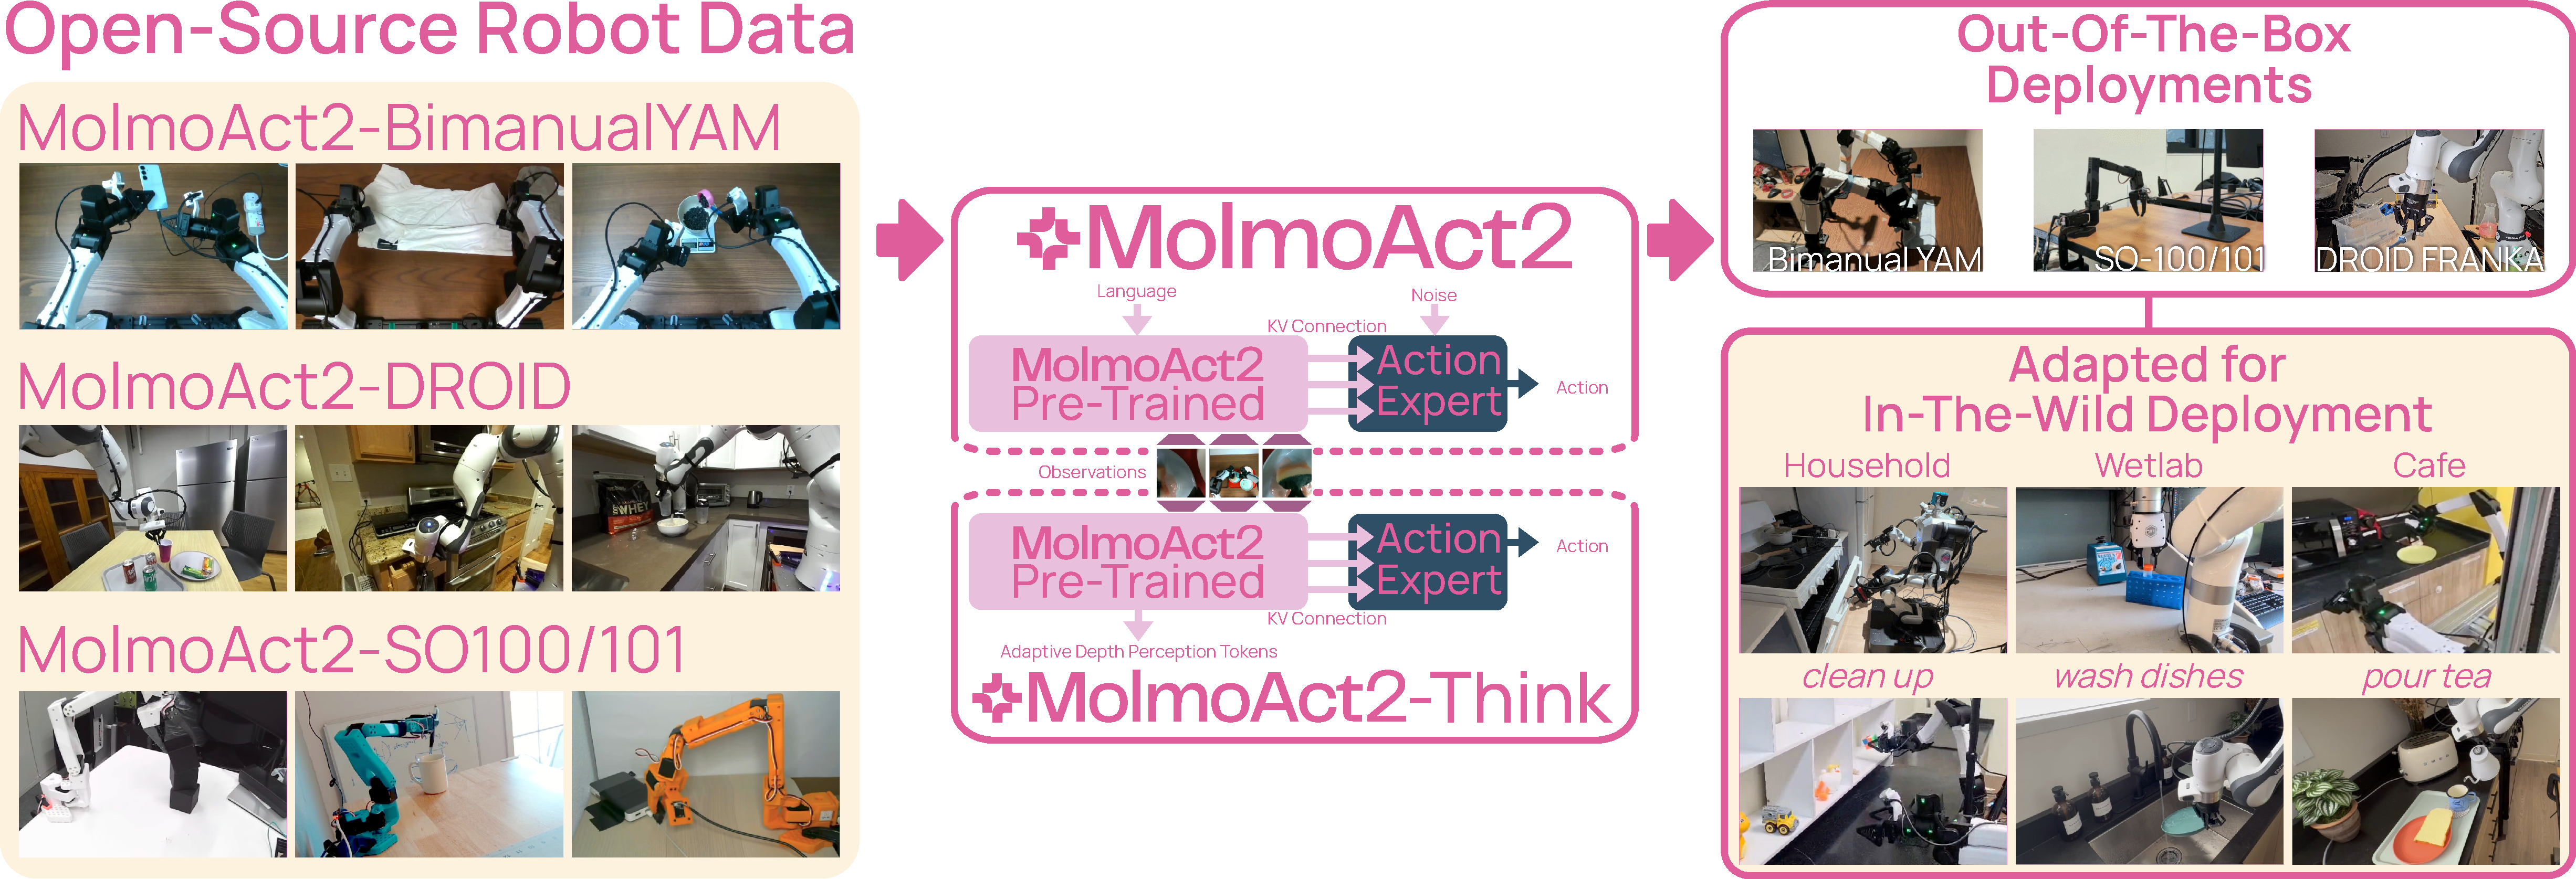
\includegraphics[width=\linewidth]{figures/MAF11.pdf}
\caption{\textbf{Overview of \molmoactt.} \molmoactt is a fully open action reasoning model for real-world deployment. From a suite of high-quality robot datasets that we collect, filter, and curate at scale across three platforms spanning the low-to-medium cost range (\textbf{left}), we train \molmoactt and its adaptive-depth reasoning variant \molmothink, coupled to the VLM backbone through per-layer KV conditioning (\textbf{center}). The resulting models deploy out-of-the-box on bimanual YAM, SO-100/101, and DROID Franka, and adapt to in-the-wild tasks such as cleaning up, washing dishes, wetlab automation, and pouring tea (\textbf{right}).}
\label{fig:teaser}
\end{figure}

We present \textbf{\molmoactt}, an action reasoning model built for real-world deployment: fully open, deployable out-of-the-box on multiple embodiments, performant, and capable of fast, interpretable reasoning (Figure~\ref{fig:teaser}). \molmoactt improves over its predecessor MolmoAct~\citep{lee2025molmoactactionreasoningmodels} along five axes vital for a strong action reasoning model: (1) a stronger open embodied-reasoning VLM backbone, (2) new open-source training datasets, (3) \molmoactfast, an open-source multi-embodiment action tokenizer, (4) a new VLA architecture design, and (5) a new adaptive reasoning paradigm for efficient inference.

First, we train \textbf{\molmoer} (Sec.~\ref{sec:er}), a VLM specialized for spatial and embodied reasoning.
General-purpose VLMs rarely train on or test the embodied skills a robot policy needs: they need to understand metric distances, free space, cross-view object tracking, and scene geometry. 
We address this by training \molmoer on a 3.3M-sample spatial–embodied corpus using a specialize-then-rehearse recipe. 

Second, existing open robot datasets remain fragmented across embodiments, uneven in quality, and too small or noisy to support reliable multi-embodiment action learning.
To support training action models on top of our VLM backbone, we release three action datasets (Sec.~\ref{sec:data}) targeting three platforms across a low-to-medium cost range: \textbf{\molmoacttyamdata}, 720 hours of teleoperated YAM trajectories spanning tabletop and household tasks—the largest open bimanual dataset to date; \textbf{\molmoacttsodata}, a filtered subset of internet SO-100/101 data with mislabeled and low-quality trajectories removed; and \textbf{\molmoacttdroiddata}, a quality-filtered Franka subset of DROID. For the two filtered datasets, we also re-annotate the language instructions for improved diversity and accuracy. 

Third, existing action tokenizers are either closed, tied to specific action spaces, or insufficiently documented, making it difficult to train reproducible discrete-action VLAs across embodiments.
To make the trajectories in our data usable under a discrete autoregressive objective, we introduce \molmoactfast, an open-weight, open-data implementation following FAST~\citep{pertsch2025fast}. We train and release its weights along with the millions of trajectories across five embodiments used to train it. \molmoactfast compresses one second of 32-D continuous actions into a compact discrete sequence.

Fourth, discrete-token VLMs provide strong reasoning grounding, but their native output space is poorly matched to the continuous, high-frequency trajectories required by robot control. A new architecture is therefore needed to connect the discrete reasoning capacity with smooth continuous actions.
We design a new architecture that conditions each layer of the continuous action expert on the keys and values from the corresponding VLM layer.
This design is in contrast to existing VLAs with action experts in two ways. First, we use a DiT-style transformer trained with flow matching objective, giving the continuous controller a modern denoising-transformer architecture that has proven more effective than many alternatives for diffusion and flow-based generative modeling. Second, instead of conditioning the expert on VLM hidden states, we condition each expert layer on the corresponding VLM keys and values. This preserves a similar compute profile while exposing the attention state used by the VLM itself, which has been shown to be more effective in our ablation studies.

Fifth, prior reasoning-based VLAs improve action quality by generating dense intermediate representations at every step~\cite{lee2025molmoactactionreasoningmodels}, but this repeats nearly identical computation across largely static scenes and makes inference too slow for real-time control.
We introduce \textbf{\molmothink}, the reasoning variant of \molmoactt, which performs \textit{adaptive} depth reasoning by autoregressively predicting only the tokens for scene regions that change between timesteps. This exploits trajectory-level temporal redundancy to reduce latency proportional to the static scene fraction while retaining the geometric grounding that significantly improves model performance.

To understand the capabilities of \molmoactt and assess its readiness for real-world deployment, we conduct the most extensive empirical study of any open VLA to date, spanning 7 environment benchmarks across both simulation and the real world. Across all of them, \molmoactt, with \molmothink, outperforms every strong baseline. We show that \molmoactt's fine-tuned checkpoints, \molmoacttdroid and \molmoacttso, can be deployed out of the box on their respective embodiments without any additional fine-tuning, significantly surpassing $\pi_{0.5}$~\citep{intelligence2025pi05visionlanguageactionmodelopenworld} (Sec.\ref{sec:exp-outbox}). We further demonstrate that \molmoactt is built on one of the strongest embodied-reasoning VLM backbones available: \molmoer surpasses models such as GPT-5~\citep{singh2025openai} and Gemini Robotics Embodied Reasoning (ER)-1.5~\citep{team2025gemini15} on 13 standard embodied-reasoning benchmarks (Sec.\ref{sec:exp-er}). 

For rapid real-world deployment via efficient fine-tuning to new embodiments, \molmoactt opens large performance gaps over strong general-purpose VLAs such as $\pi_{0.5}$~\citep{intelligence2025pi05visionlanguageactionmodelopenworld} not only on the two mainstream simulation benchmarks LIBERO~\citep{liu2023libero} and RoboEval~\citep{wang2025roboeval}, but also on a comprehensive evaluation suite of 8 real-world tasks on the bimanual YAM setup (Sec.\ref{sec:exp-ft}). Our ablations demonstrate that \molmothink models yield further gains over \molmoactt while providing additional interpretability that aids both diagnosis and performance (Sec.\ref{depth}).

\molmoactt is fully open in every respect, and beyond that, is capable of supporting real-world deployment for practical tasks: we release the model weights, training code, and the complete training dataset. We aim for \molmoactt to be more than an academic robotics foundation model; we want it to be a model that can be deployed in real-world workflows and deliver meaningful social impact.

\section{Related Work}
\label{sec:related}

Group related work into 2--4 themes, one paragraph each, and end every paragraph by saying how your work differs. Do not just list papers.

\paragraph{Citations.} The template uses \texttt{natbib} with author--year citations. Use \verb|\citep| for parenthetical citations, e.g.\ vision-language-action models~\citep{kim2024openvla,black2410pi0}, and \verb|\citet| when the authors are part of the sentence, e.g.\ \citet{khazatsky2024droid} collected a large in-the-wild dataset. Always put a non-breaking space (\verb|~|) before \verb|\citep|.

\paragraph{Bibliography.} Add entries to \texttt{reference.bib}. Prefer the published version (conference or journal) of a paper over its arXiv version, and keep entry keys consistent, e.g.\ \texttt{lastnameYEARfirstword}.

\section{Methodology}
\label{sec:method}

Describe \methodname{}. Introduce notation, define the problem formally, and then
present your approach. Number important equations so you can reference them, e.g.
\cref{eq:objective}:
\begin{equation}
    \mathcal{L}(\theta) = \frac{1}{N} \sum_{i=1}^{N}
        \ell\big(f_\theta(x_i),\, y_i\big).
    \label{eq:objective}
\end{equation}

\subsection{Component One}
\label{subsec:component-one}
Explain the first component of your method. Figures live under \texttt{figures/}
and are included with \texttt{\textbackslash includegraphics}. \cref{fig:overview}
shows a single-image figure.

\begin{figure}[t]
    \centering
    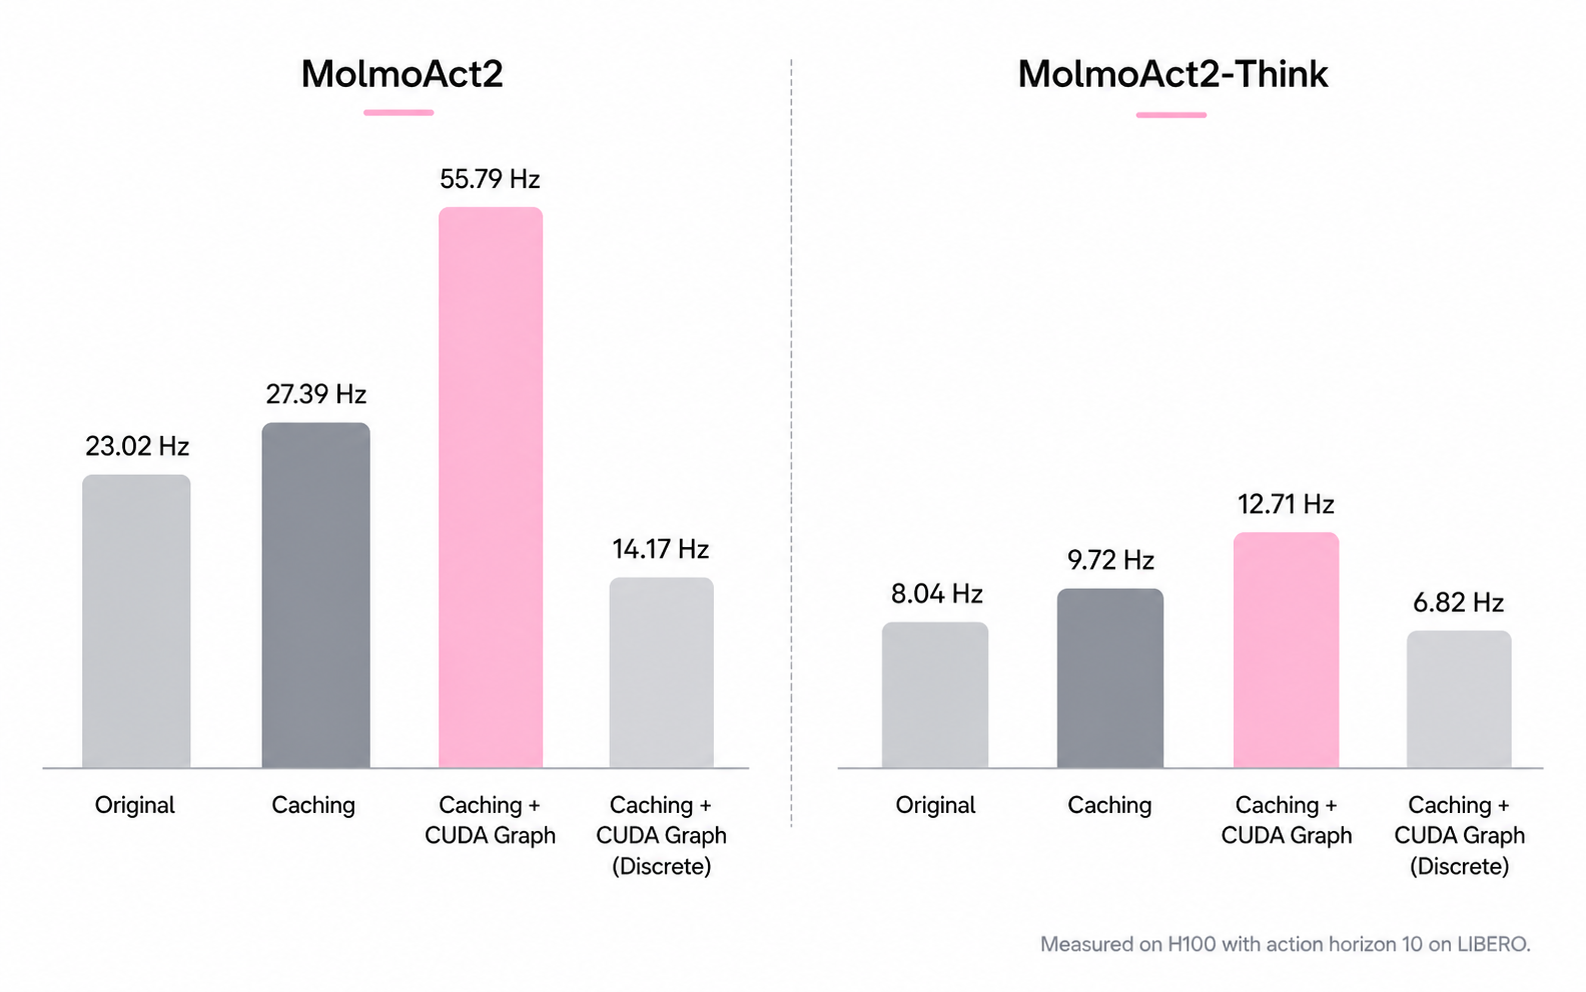
\includegraphics[width=0.7\linewidth]{figures/example_plot.png}
    \caption{\textbf{Single figure.} Replace \texttt{figures/example\_plot.png}
    with your own image. Use \texttt{width=...\textbackslash linewidth} to scale
    relative to the text width.}
    \label{fig:overview}
\end{figure}

\subsection{Component Two}
\label{subsec:component-two}
Explain the second component and how it connects to the first. Use
\texttt{subcaption} for multi-panel figures; reference a panel with
\cref{fig:panel-a} or the whole figure with \cref{fig:panels}.

\begin{figure}[t]
    \centering
    \begin{subfigure}{0.48\linewidth}
        \centering
        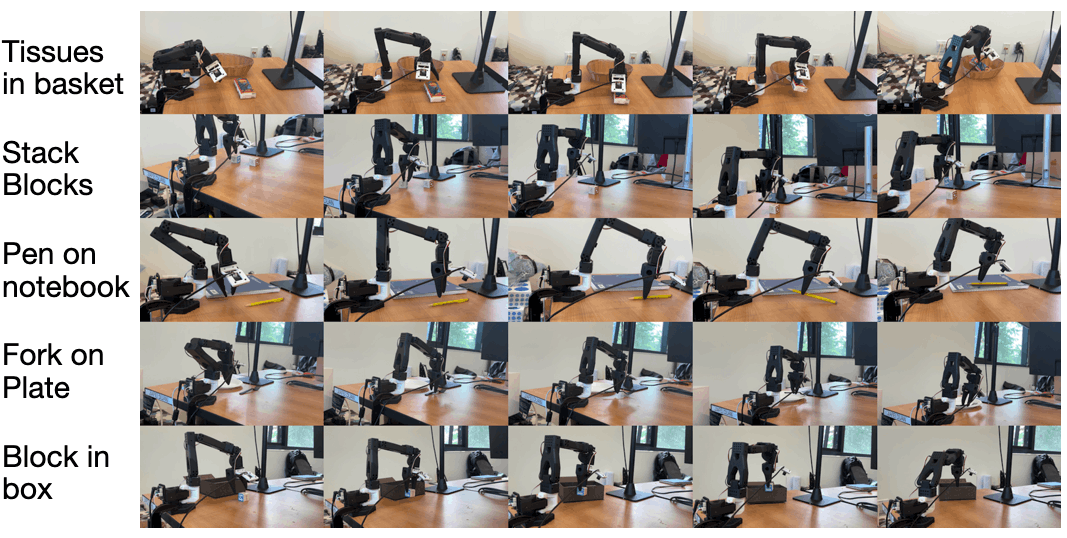
\includegraphics[width=\linewidth]{figures/example_panel_a.png}
        \caption{First panel.}
        \label{fig:panel-a}
    \end{subfigure}
    \hfill
    \begin{subfigure}{0.48\linewidth}
        \centering
        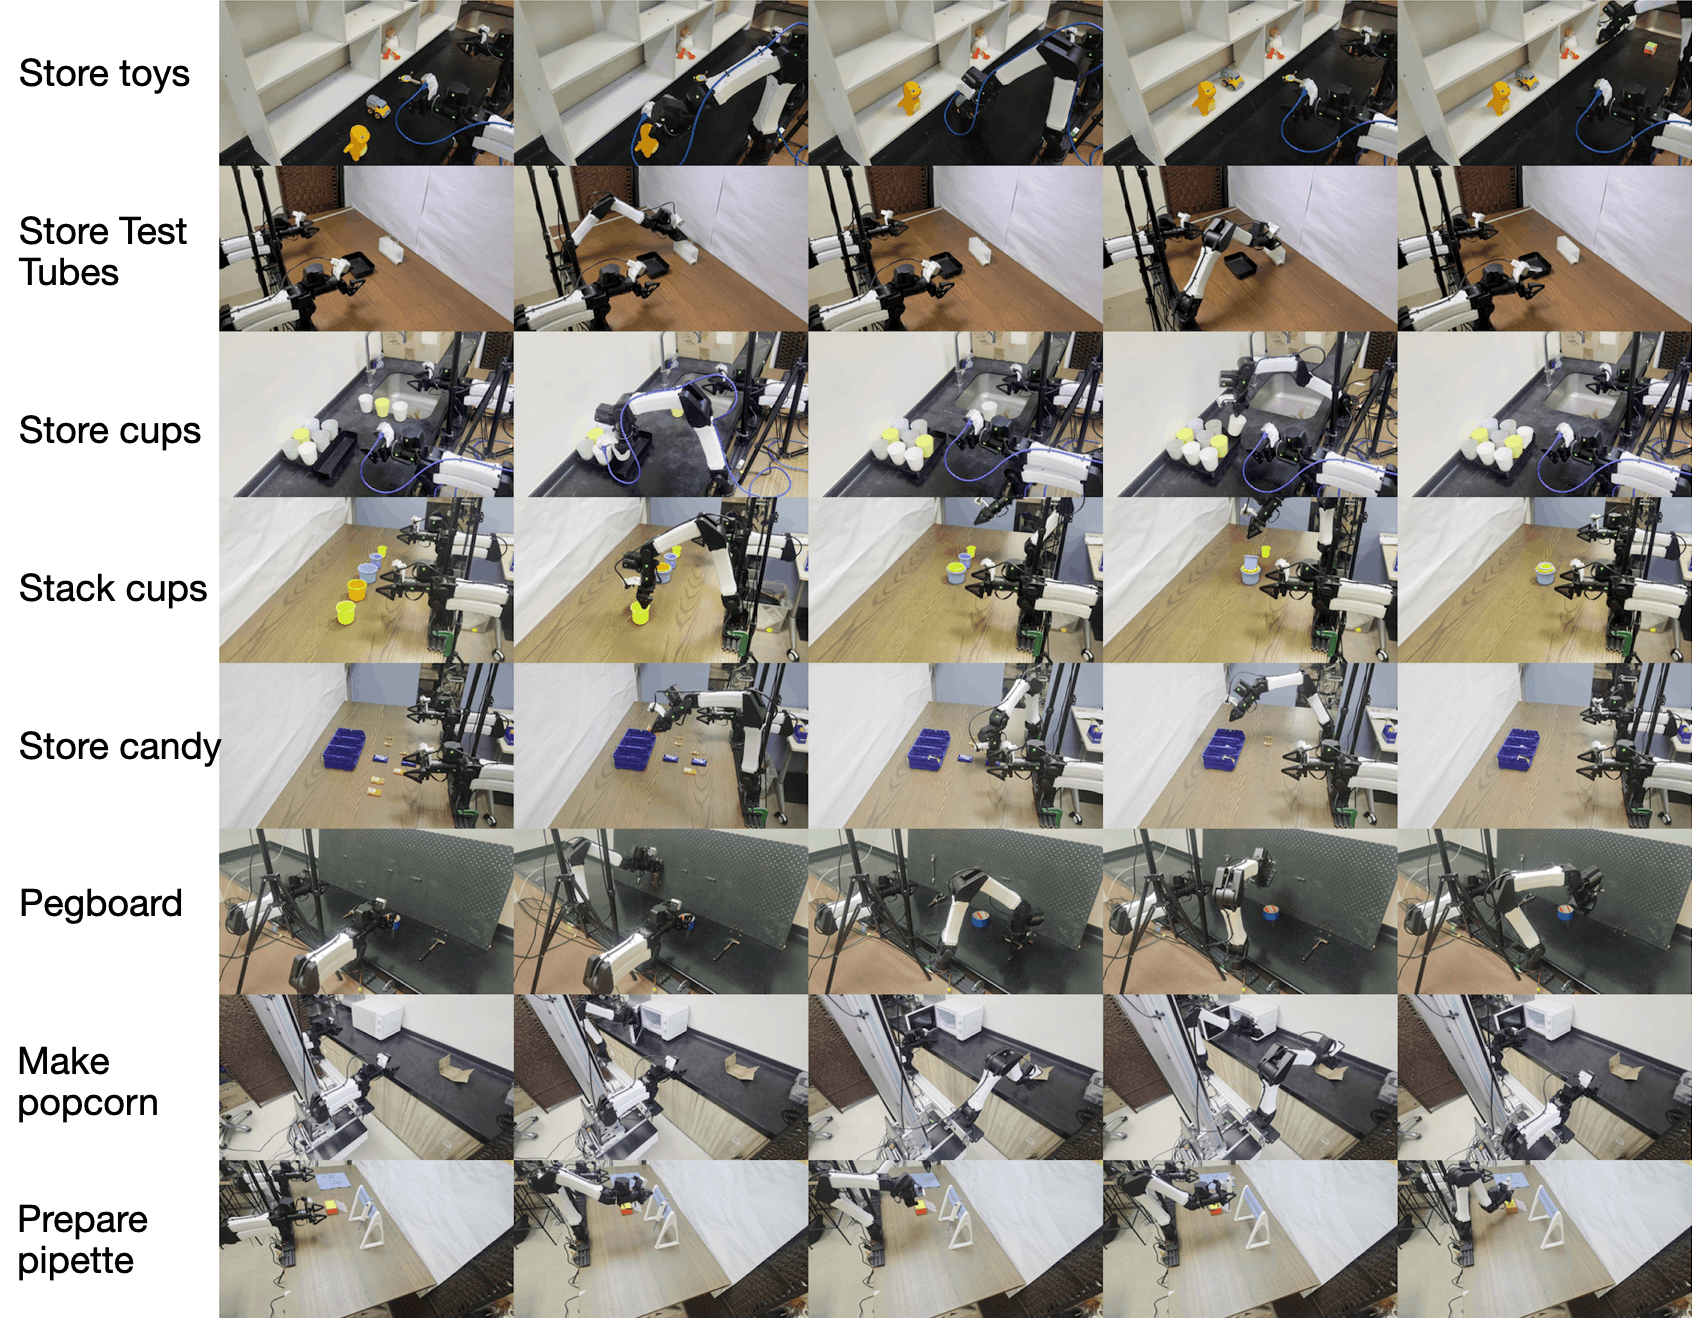
\includegraphics[width=\linewidth]{figures/example_panel_b.png}
        \caption{Second panel.}
        \label{fig:panel-b}
    \end{subfigure}
    \caption{\textbf{Two-panel figure.} Side-by-side images via the
    \texttt{subfigure} environment, each with its own sub-caption and label.}
    \label{fig:panels}
\end{figure}


\section{Evaluation}
\label{sec:evaluation}

Describe your experimental setup: datasets, baselines, metrics, and
implementation details. State the research questions your experiments answer.

\subsection{Experimental Setup}
\label{subsec:setup}
Specify datasets, baselines, metrics, and training/evaluation details so your
results are reproducible.

\subsection{Main Results}
\label{subsec:results}
Report and discuss your main results. \cref{tab:main-results} shows an example
results table that is kept in its own file under \texttt{tables/} and pulled in
here with \texttt{\textbackslash input\{tables/main\_results\}}.

% Sample results table kept in its own file under tables/ and pulled into the
% evaluation section with % Sample results table kept in its own file under tables/ and pulled into the
% evaluation section with \input{tables/main_results}. Keeping tables in a
% separate folder keeps your section prose readable.
\begin{table}[t]
    \centering
    \begin{tabular}{lcc}
        \toprule
        Method & Metric A $\uparrow$ & Metric B $\uparrow$ \\
        \midrule
        Baseline A           & 70.0          & 61.2 \\
        Baseline B           & 74.3          & 68.0 \\
        \methodname{} (ours) & \textbf{82.5} & \textbf{74.8} \\
        \bottomrule
    \end{tabular}
    \caption{\textbf{Main results.} Bold marks the best result per column.
    Replace with your own numbers and add standard errors where appropriate.}
    \label{tab:main-results}
\end{table}
. Keeping tables in a
% separate folder keeps your section prose readable.
\begin{table}[t]
    \centering
    \begin{tabular}{lcc}
        \toprule
        Method & Metric A $\uparrow$ & Metric B $\uparrow$ \\
        \midrule
        Baseline A           & 70.0          & 61.2 \\
        Baseline B           & 74.3          & 68.0 \\
        \methodname{} (ours) & \textbf{82.5} & \textbf{74.8} \\
        \bottomrule
    \end{tabular}
    \caption{\textbf{Main results.} Bold marks the best result per column.
    Replace with your own numbers and add standard errors where appropriate.}
    \label{tab:main-results}
\end{table}


\subsection{Ablations}
\label{subsec:ablations}
Isolate the effect of each component to justify your design choices.

\section{Conclusion}
\label{sec:conclusion}

Summarize the problem, the method, and the main findings in one short paragraph. Do not repeat the abstract word for word.

\paragraph{Limitations.} Many robotics venues (e.g.\ CoRL) require an explicit limitations section. Be honest and specific: describe the failure modes you observed, the assumptions \method makes (e.g.\ known camera calibration, a fixed embodiment), and what is left for future work.


%%%%% ACKNOWLEDGMENT %%%%%
% Acknowledgments are typically not anonymized only in the camera-ready version.
\section*{Acknowledgments}
\label{sec:ack}

Thank collaborators, funding sources, and compute providers here. For MAGIC Lab
work, acknowledge the National University of Singapore, School of Computing, and
any grants or hardware that supported the project.


%%%%%%%%% REFERENCES %%%%%%%%%
\clearpage
\bibliographystyle{abbrvnat}
\bibliography{reference}

%%%%%%%% APPENDIX %%%%%%%%%
\clearpage
\beginappendix

\section{Implementation Details}
\label{app:implementation}

Put material that supports the main paper but is not needed to follow it here: hyperparameters, network details, full task descriptions, additional results, and failure cases. Refer to each appendix section from the main text, e.g.\ ``see \cref{app:implementation}''.

\section{Additional Results}
\label{app:results}

Additional tables and figures go here.


\end{document}
